\documentclass[12pt]{report}

%Packages-------------------------------------
\usepackage{amsmath}
\usepackage{amsfonts}
\usepackage{amssymb}
\usepackage{amsthm}
\usepackage{graphics}
\usepackage{graphicx}
\usepackage{hyperref}
\usepackage{listings}
\usepackage{xepersian}
%\usepackage{xtocnic}

\settextfont{XB Zar}

\lstset{
    basicstyle=\ttfamily\small,
    language=Python,
    numbers=left,
    numberstyle=\tiny\lr,
    showstringspaces=false,
    columns=fullflexible
}

%Layout---------------------------------------

%\usepackage[top=2cm, bottom=2cm, left=2cm, right=2cm]{geometry}

%Commands-------------------------------------


%Theorems-------------------------------------
\newtheorem{thm}{قضیه}[chapter]
\newtheorem{cor}[thm]{نتیجه}
\newtheorem{defn}[thm]{تعریف}
\newtheorem{prop}[thm]{گزاره}
\newtheorem{lmm}[thm]{لم}
\newtheorem{conj}[thm]{حدس}
\newtheorem{exm}[thm]{مثال}
\newtheorem{rem}[thm]{تذکر}
\newtheorem{note}[thm]{یادداشت}
\newtheorem{alg}[thm]{الگوریتم}


\begin{document}

%Title page ---------------------------------------------

\begin{figure}
\centering

\includegraphics[height=2.5cm]{UT-Logo.pdf}
\end{figure}

\begin{center}
پردیس علوم
\\
دانشکده ریاضی، آمار و علوم کامپیوتر
\end{center}

\begin{center}
%%%%%%%%%%%%%
\end{center}

\begin{center}
\huge{آشنایی با الگوریتم‌های تکرار بافاصله: چگونه فلش‌کارت‌ها به مقابله با فراموشی کمک می‌کنند؟}
\end{center}

\begin{center}
%%%
\end{center}

\begin{center}
نگارنده
\end{center}
\begin{center}
\textbf{
محمد ترابی}
\end{center}

\begin{center}
\begin{tabular}{rr}
استاد راهنما: دکتر هدیه ساجدی

\end{tabular}
\end{center}

\vspace{3cm}
\begin{center}
پایان‌نامه برای دریافت درجه کارشناسی
\\
در رشته علوم کامپیوتر
\end{center}

\begin{center}
تاریخ: شهریور ۱۴۰۴
\end{center}

\pagestyle{empty}
\pagenumbering{}

\newpage
%\pagestyle{headings}
%\setcounter{page}{1}
%\pagenumbering{roman}
\pagestyle{plain}
\setcounter{page}{1}
\pagenumbering{harfi}
%Abstract page-------------------------------
\chapter*{}

\section*{چکیده}
این مقاله به کاوش در مکانیزم‌های بهبود حافظه از طریق 
فلش‌کارت‌ها و رویکرد \textbf{تکرار بافاصله} می‌پردازد. 
ابتدا، مفهوم \textbf{منحنی فراموشی} و پیامدهای 
آن برای یادگیری تشریح می‌شود. سپس، با معرفی 
ویژگی‌های یک فلش‌کارت مؤثر ، به بررسی اصول 
شناختی پشت این ابزار پرداخته می‌شود. در بخش 
اصلی، \textbf{ویژگی‌های کلیدی الگوریتم‌های تکرار بافاصله} 
(مانند بهینه‌سازی فواصل و توزیع بار مرور) 
مورد بحث قرار گرفته و دو الگوریتم مهم 
یعنی \lr{Leitner} و \lr{SuperMemo} به تفصیل بررسی می‌شوند.
در نهایت، با استناد به یافته‌های تحقیقاتی و آزمایشات وزنیاک، این پژوهش بر اهمیت طراحی الگوریتم‌های بهینه برای مدیریت مؤثر فرآیند یادگیری تاکید می‌کند.

% \chapter*{تقدیم به}
% تمام انسان‌هایی که تا به حال در قسمت تقدیم به نبودند!
%\section*{تقدیم به}

%Acknowledgement page------------------------
\chapter*{سپاسگزاری}
صمیمانه از استاد راهنمای گرانقدرم، سرکار خانم دکتر ساجدی، برای تدریس، راهنمایی‌ها و‌ حمایت‌های ارزشمندشان سپاسگزارم. از جناب آقای دکتر باباعلی، مدیر محترم گروه، نیز بابت زحمات و آموزه‌های گران‌قدرشان کمال تشکر را دارم. یاد و خاطرهٔ استاد ارجمند، مرحوم دکتر نوذری، که دانش و بینش ایشان همواره الهام‌بخش بود، گرامی باد.

%copyright + declaration page
%\chapter*{اصالت اثر}
%\section*{اصالت اثر}
% هیچ قسمت از این پایان‌نامه، پیش از این در هیج موسسه تحصیلات عالی برای دریافت درجه تحصیلی استفاده نشده است. همچنین، هیچ قسمت از این پایان‌نامه برگردان فارسی تمامی یا قسمتی از یک اثر دیگر علمی (مانند مقاله، پایان‌نامه، و غیره) به زبانی دیگر نمی‌باشد. ارائه این پایان‌نامه توسط نگارنده به معاونت آموزشی (معاونت پژوهشی و تحصیلات تکمیلی برای ارشد و دکتری) به منزله تعهد نگارنده به اصالت متن و محتوای ارائه شده بر اساس یک کار پژوهشی در مدت تحصیل در دانشگاه تهران می باشد. در صورت اثبات خلاف این امر، مدرک تحصیلی اخذ شده توسط این پایان‌نامه از دانشگاه تهران، معتبر نمی باشد. 
%
%\chapter*{حق مالکیت معنوی}
%\section*{حق مالکیت معنوی}
%حق مالکیت معنوی این اثر متعلق به دانشگاه تهران می باشد. استفاده از مطالب این پایان‌نامه در فعالیت های تحقیقاتی با ذکر منبع بلامانع می‌باشد. در صورت استفاده تجاری، مانند چاپ این پایان‌نامه، هماهنگی لازم و اجازه کتبی از دانشگاه و نگارنده پایان‌نامه الزامی می‌باشد.

%\listoffigures

%-------------------------
%\pagestyle{plain}
%\setcounter{page}{1}
%\pagenumbering{harfi}
%-------------------------

\chapter*{پیشگفتار}

یکی از چالش‌های بنیادین در فرآیند یادگیری، مقابله با پدیده طبیعی فراموشی است. از زمان پژوهش‌های پیشگامانه‌ای چون \lr{Hermann Ebbinghaus} در حوزه \textbf{منحنی فراموشی}، همواره این سوال مطرح بوده است که چگونه می‌توان اطلاعات را به شکلی مؤثر و ماندگار در حافظه ذخیره کرد. این پژوهش، در تلاش برای ارائه پاسخی علمی به این سوال، به بررسی رویکردهای نوین در حوزه بهینه‌سازی فرآیند یادگیری می‌پردازد. در این راستا، \textbf{فلش‌کارت‌ها} به عنوان ابزاری قدرتمند و روش \textbf{تکرار بافاصله} به عنوان راهکاری علمی برای مبارزه با فراموشی، مورد توجه قرار گرفته‌اند.

تلاش‌های نخستین در این زمینه با ابداع سیستم‌هایی چون روش \lr{Leitner} آغاز شد و در ادامه، با توسعه الگوریتم‌های پیشرفته‌تری مانند \lr{SuperMemo} توسط «\lr{Piotr Woźniak}»، این حوزه وارد فاز جدیدی از دقت و کارایی گردید. هدف از این پژوهش، ارائه یک تحلیل جامع از اصول، مزایا و محدودیت‌های این روش‌هاست تا اهمیت رویکرد الگوریتمی در تقویت حافظه آشکار گردد.

ساختار این پژوهش به گونه‌ای است که ابتدا مبانی نظری و علمی موضوع را تبیین می‌نماید. در ادامه، اصول طراحی فلش‌کارت‌های مؤثر و الگوریتم‌های کلیدی تکرار بافاصله مورد بررسی قرار می‌گیرد. همچنین نسخه نرم‌افزاری این سیستم‌ها به عنوان پیاده‌سازی عملی این پژوهش توسعه یافته است.
کد منبع این پروژه و مستندات مربوط به آن را می‌توانید در مخزن گیت‌هاب مربوطه به آدرس
\href{https://github.com/mitinull/spaced-repetition-lab}{github.com/mitinull/spaced-repetition-lab}
مشاهده کنید.

\tableofcontents

\chapter{مفاهیم مقدماتی}

%---------------------
\pagestyle{plain}
\setcounter{page}{1}
\pagenumbering{arabic}
%---------------------


% یک پایان‌نامه ریاضی، معمولاً شامل تعاریف و مفاهیم تخصصی می‌باشد. توصیه می‌شود که فصلی از پایان‌نامه به معرفی مفاهیم مقدماتی که در پایان‌نامه به کار رفته‌اند اختصاص یابند. معمولاً نمادگذاری و معرفی کلیدواژه‌های به کار رفته در پایان‌نامه در این فصل انجام می‌پذیرد و یک خواننده عادی، داور پایان‌نامه، یا هر شخص دیگری در صورت عدم آشنایی با مفهومی می‌تواند به این فصل مراجعه نماید. توصیه می‌کنیم که این معرفی و نمادگذاری به زبانی روان و گویا انجام پذیرد و نیز با توجه به تفیکیک موصوعات و ارتباط منطقی بین آنها انجام پذیرد. معمولاً هر فصل، به غیر از پیشگفتار، شامل بخش‌ها و زیر بخش‌هایی می‌باشد که می‌توانند بر اساس تقسیم‌بندی موضوعی صورت پذیرند. برای نمونه برای مطالعه یک مطلب درباره سیستم‌های دینامیکی ناخودگرد، وجود یک بخش درباره سیستم‌های دینامیکی در حالت کلی و نیز بخش یا زیربخشی درباره حالت ناخودگردی یک تقسیم‌بندی مناسب به نظر می‌آید.

% توجه کنید که لزومی به اثبات همه مطالب و قضیه‌های مقدماتی، در این فصل، نیست و اصولاً چنین کاری شیوه مرسوم نیست. معمولاً انتخاب و ارجاع خواننده به یک کتاب معتبر یا هر مرجع معتبر دیگری بسیار مناسب‌تر است. چنین فصلی، جایی مناسب برای قضیه‌های "کلاسیک" درباره مساله مورد مطالعه می‌باشد. توجه کنید که یک قضیه می‌تواند صورت‌های مختلفی داشته باشد و بهتر است از آن صورت مورد استفاده خود در این قسمت استفاده نمایید!

\section{فلش‌کارت}
فلش‌کارت‌ها ابزاری ساده اما بسیار 
\textbf{کارآمد}
برای یادگیری و به‌خاطرسپاری اطلاعات هستند. این ابزارها، که می‌توانند به شکل 
کاغذی یا الکترونیکی باشند، شامل مجموعه‌ای از کارت‌ها هستند
 که روی یک یا هر دو طرف آن‌ها اطلاعاتی نوشته شده است. از فلش‌کارت‌ها 
می‌توان برای یادگیری طیف گسترده‌ای از موضوعات استفاده کرد، از جمله:

\begin{itemize}
  \item \textbf{زبان‌های خارجی}: یادگیری واژگان جدید، مرور اشکال مختلف افعال بی‌قاعده
  \item \textbf{علوم پایه}: به‌خاطر سپردن مطالب در دروس پزشکی، شیمی، حقوق، تاریخ و جغرافیا
  \item \textbf{مهارت‌های تخصصی}: حفظ نت‌های گیتار، اصطلاحات علوم کامپیوتر
  \item \textbf{موارد روزمره}: مرور یادداشت‌های مهم، حفظ کردن شماره تلفن یا شماره کارت، به‌خاطر سپردن نام افراد از روی تصویرشان
\end{itemize}

\section{تکرار بافاصله
\protect\footnote{\lr{Spaced Repetition}}
}

برای ماندگاری بیشتر اطلاعات در حافظه، مرور مطالب ضروری است.
\textbf{تکرار بافاصله}
 روشی است که در آن مرور مطالب در فواصل زمانی مشخص و بهینه انجام می‌شود.
  این فواصل با گذشت زمان،
  به‌تدریج طولانی‌تر می‌شوند. 
 این شیوه بر اساس الگوریتم‌هایی 
 طراحی شده است که بهترین زمان را
  برای تکرار هر مطلب محاسبه می‌کنند. 
 با استفاده از این روش، اثربخشی
  یادگیری به‌طور چشمگیری افزایش می‌یابد. 
 در این مقاله چند الگوریتم مرتبط
  با تکرار بافاصله را 
 بررسی خواهیم کرد.

% در یک پایان‌نامه ریاضی، انواع گزاره‌ها برای بیان مطالب و مفاهیم به کار می‌رود. عناوینی مانند، قضیه، گزاره، لم، حکم، الگوریتم، اثبات، مثال، تذکر، یادآوری، یادداشت، حدس و غیره. توصیه اکید می‌کنیم که از صورت کلی زیر برای ایجاد محیط مناسب استفاده نمایید
% \begin{latin}
% \[
% \begin{array}{l}
% \backslash\textrm{begin\{env. name\}}\\
% \\
% \backslash\textrm{end\{env. name\}}
% \end{array}
% \]
% \end{latin}
% در زیر جدولی از محیط های تعریف شده آمده است

% \begin{center}
% \begin{tabular}{c|c}
% محیط تعریف شده & env. name
% \\

% \hline

% \\
% قضیه& thm
% \\
% گزاره یا حکم & prop
% \\
% لم & lmm
% \\
% تعریف & defn
% \\
% مثال & exm
% \\ 
% تذکر & rem
% \\ 
% یادداشت & note
% \\
% الگوریتم & alg
% \\
% اثبات & proof
% \end{tabular}
% \end{center}

% برای نمونه تعریف زیر با استفاده از محیط 
% $$\begin{array}{l}
% \backslash\textrm{begin\{defn\}} \\ \\
% \backslash\textrm{end\{defn\}}
% \end{array}$$
% ایجاد شده است.
% \begin{defn}
% عدد طبیعی 
% $p$، 
% $p\neq 1$، 
% را اول گوییم، هرگاه به غیر از خودش و یک مقسوم علیه دیگری نداشته باشد.
% \end{defn}

\section{منحنی فراموشی \protect\footnote{\lr{Forgetting Curve}}}
\textbf{منحنی فراموشی}
نموداری است که نشان می‌دهد چگونه میزان به‌خاطرآوردن 
مطالب در طول زمان کاهش می‌یابد.
 این نمودار توسط روانشناس آلمانی،
 هرمان ابینگهاوس
\footnote{\lr{Hermann Ebbinghaus (1850–1909)}}
 ، معرفی شد. محور 
افقی این نمودار نشان‌دهنده زمان و
 محور عمودی آن،
\textbf{میزان یادآوری}
\footnote{Retention} یا احتمال به‌خاطرآوردن مطلب است.

همانطور که در
شکل~\ref{fig:forgetting-curve}
مشخص است، اگر مطالب مرور نشوند،
 میزان یادآوری به‌سرعت کاهش می‌یابد.
 اما با استفاده از تکرار بافاصله،
 همانطور که در
شکل~\ref{fig:forgetting-curve-with-repetition}
 دیده می‌شود،
 شیب منحنی پس از هر بار مرور کمتر می‌شود.
 این بدان معناست که با هر بار تکرار،
 مدت‌زمان بیشتری طول می‌کشد تا مطلب فراموش شود
 و نیاز به مرور کمتری پیدا می‌کند.
 
\begin{figure}[h!]
  \centering
  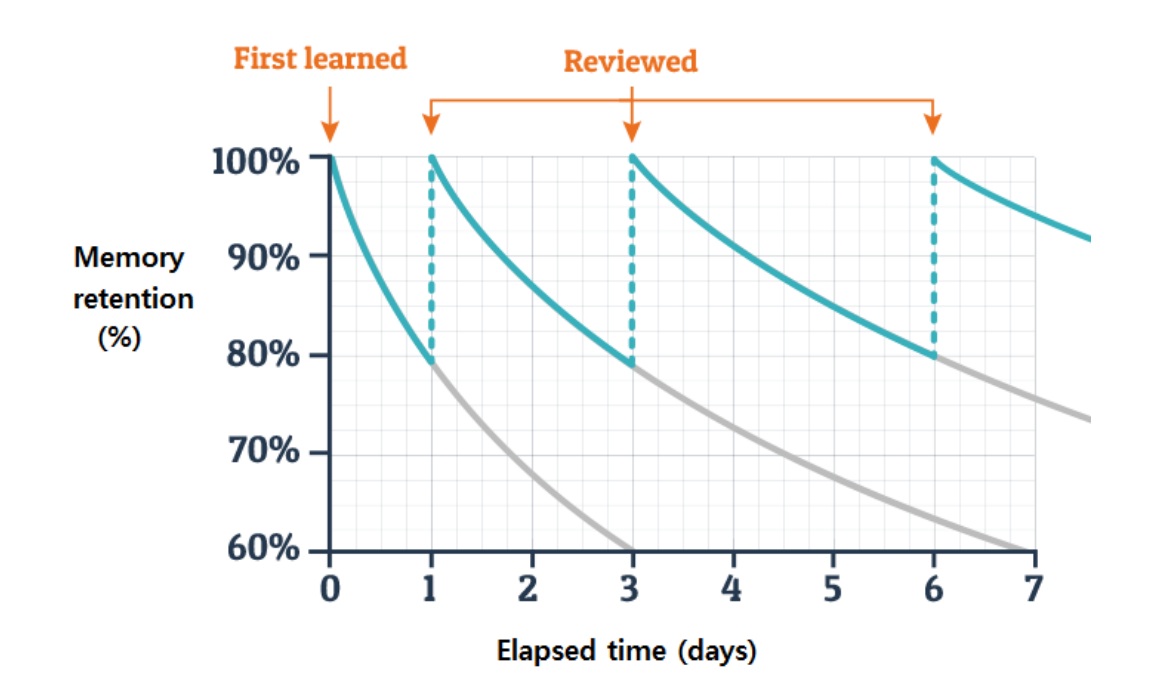
\includegraphics[width=0.8\textwidth]{images/forgetting-curve.png}
  \caption{منحنی فراموشی بدون مرور مطالب}
  \label{fig:forgetting-curve}
\end{figure}

\begin{figure}[h!]
  \centering
  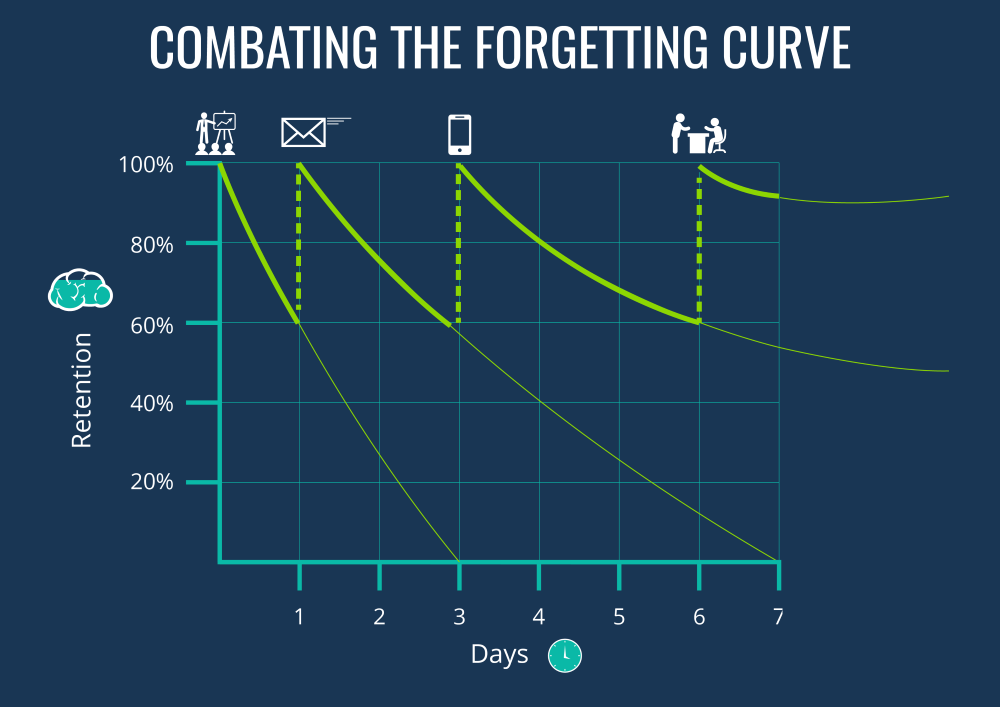
\includegraphics[width=0.8\textwidth]{images/forgetting-curve-with-repetition.png}
  \caption{منحنی فراموشی با مرور مطالب}
  \label{fig:forgetting-curve-with-repetition}
\end{figure}

\chapter{اصول طراحی فلش‌کارت‌های کارآمد}


\section{ویژگی‌های یک فلش‌کارت خوب}

% ایجاد لیست شماره‌دار با استفاده از محیط enumerate
    \subsubsection{طراحی به شکل پرسش و پاسخ:} بهترین فلش‌کارت‌ها از شما می‌خواهند به جای مرور صرف، به یک سوال پاسخ دهید. تحقیقات نشان داده‌اند که \textbf{یادآوری فعال}\footnote{\lr{Active Recall}}، یعنی تلاش برای بازیابی اطلاعات، به یادگیری عمیق‌تر و ماندگارتر منجر می‌شود. این پدیده به «\textbf{اثر آزمون}»\footnote{\lr{Testing Effect}} نیز معروف است.

    \subsubsection{کوتاه و مختصر:} یک فلش‌کارت باید شامل یک مفهوم یا واقعیت واحد باشد. مطالب کوتاه‌تر، یادگیری را ساده‌تر کرده و امکان مرور متناسب با میزان سختی هر بخش را فراهم می‌کنند. در مقابل، کارت‌های شلوغ مجبورمان می‌کنند کل محتوا را تکرار کنیم، حتی اگر بخشی از آن را بلد باشیم.

    \subsubsection{اجتناب از فهرست‌ها:} به جای پرسیدن "کشورهای خاورمیانه را نام ببرید؟"، بهتر است هر کشور را در یک کارت جداگانه با سوالات خاصی مانند "بزرگ‌ترین کشور خاورمیانه کدام است؟" یا "ثروتمندترین کشور آن کدام است؟" یاد بگیرید. این کار از ناکارآمدی حفظ فهرست‌های بلند جلوگیری می‌کند. سپس می‌توانید با پیوند دادن این اطلاعات، به سوال اصلی پاسخ دهید.
    
    \subsubsection{منابع بیشتر:} برای آشنایی با ویژگی‌های دقیق‌تر و قوانین بهینه‌سازی فلش‌کارت‌ها، می‌توانید به مقالهٔ 
    «\href{https://super-memory.com/articles/20rules.htm}{بیست قانون برای فرمول‌بندی دانش}»
\cite{20rules}
    مراجعه کنید. این مقاله توسط پاوو اولکوفسکی، بنیان‌گذار الگوریتم \lr{SuperMemo}، نوشته شده است.

\section{مزایا و معایب مطالعه با فلش‌کارت‌ها}


\subsection*{مزایا:}
\begin{itemize}
    \item \textbf{افزایش ماندگاری:} با استفاده از تکرار بافاصله، مطالب برای مدت‌زمان طولانی‌تری در حافظه می‌مانند.
    \item \textbf{یادگیری فعال:} فلش‌کارت‌ها به دلیل ماهیت پرسش و پاسخ خود، یادگیری را فعال کرده و به جای مرور صرف، به یادآوری و بازیابی اطلاعات کمک می‌کنند.
    \item \textbf{تمرکز بر نقاط ضعف:} با طبقه‌بندی کارت‌ها بر اساس میزان سختی، می‌توان روی مطالبی که تسلط کمتری بر آن‌ها دارید، بیشتر تمرکز کرد.
    \item \textbf{بازی سازی\footnote{\lr{Gamification}}:} افزایش جذابیت و انگیزه در یادگیری به دلیل ساده 
    و بازی‌گونه بودن فلش‌کارت‌ها.
     همچنین آمارها، تحلیل‌ها و مصور سازی
      میزان پیشرفت مطالعه به ادامه دار شدن یادگیری کمک می‌کند.
\end{itemize}

\subsection*{معایب:}
\begin{itemize}
    \item \textbf{زمان‌بر بودن:} تهیه فلش‌کارت‌ها ممکن است زمان‌بر باشد، هرچند ابزارهای الکترونیکی این فرایند را ساده‌تر کرده‌اند.
    \item \textbf{نیاز به نظم و انضباط:} اثربخشی این روش به مرور منظم و مداوم وابسته است.
\end{itemize}

\chapter{اصول طراحی الگوریتم‌های تکرار بافاصله}

\section{ویژگی‌های کلیدی یک الگوریتم تکرار موثر}
% یک الگوریتم تکرار خوب، برای بهینه‌سازی فرآیند یادگیری، باید ویژگی‌های زیر را داشته باشد. 
% هدف بیشتر پژوهش‌ها در این زمینه این است که الگوریتمی طراحی شود که بتواند این ویژگی‌ها را به بهترین شکل ممکن پیاده‌سازی کند.
% البته جمع شدن همه این ویژگی‌ها در یک الگوریتم کار راحتی نیست.

هدف بیشتر پژوهش‌ها در زمینه فلش‌کارت‌ها و تکرار بافاصله این است که
الگوریتمی طراحی  شود که بهترین تاثیر را در یادگیری داشته باشد.
این هدف نیازمند داشتن ویژگی‌های متعددی‌ست که جمع شدن همه آن‌ها در یک الگوریتم کار راحتی نیست.
برخی از مهم‌ترین ویژگی‌های یک الگوریتم تکرار موثر در ادامه آمده است:

\subsubsection{محاسبه بهینه فواصل تکرار:} هدف اصلی الگوریتم، یافتن \textbf{بهترین زمان تکرار} برای هر کارت است. این زمان باید طوری باشد که کارت درست قبل از اینکه فراموش شود، دوباره نمایش داده شود. این کار باعث می‌شود با \textbf{کمترین تعداد مرور}، اطلاعات برای \textbf{بیشترین زمان ممکن} در حافظه باقی بماند.

\subsubsection{توزیع بار مرور:} یک الگوریتم هوشمند باید از \textbf{انباشته شدن فلش‌کارت‌ها} در یک روز خاص جلوگیری کند. به عبارت دیگر، وظیفه آن \textbf{توزیع بهینه} کارت‌ها در طول زمان است تا کاربر هر روز حجم معقول و مدیریت‌پذیری از کارت‌ها را برای مرور داشته باشد و از احساس خستگی یا عقب‌افتادگی جلوگیری شود. یعنی حجم فلش‌کارت‌ها در یک روز نباید خیلی کم و یا خیلی زیاد باشد.

\subsubsection{تطبیق با سختی مطالب:} الگوریتم باید بر اساس عملکرد کاربر و \textbf{سختی و آسانی} هر کارت، فواصل تکرار را تنظیم کند. برای کارت‌های آسان‌تر، فاصله زمانی بیشتر می‌شود و برای کارت‌های دشوار، مرور در فواصل کوتاه‌تری انجام می‌گیرد. این ویژگی، فرآیند یادگیری را شخصی‌سازی کرده و کارآمدتر می‌کند.

\subsubsection{سازگاری با مطالعه نامنظم:} یک الگوریتم قوی باید با \textbf{مطالعه نامنظم} سازگار باشد و در صورت وقفه طولانی، دچار اختلال نشود. اگر کاربری برای چند روز یا هفته مطالعه نکند و سپس مرور را از سر بگیرد، الگوریتم باید این وقفه را درک کرده و فواصل زمانی را به‌درستی تنظیم کند. برای مثال، اگر قرار بود کارتی امروز مرور شود و سپس یک هفته بعد نمایش داده شود اما کاربر به جای امروز پس از یک ماه آن را مرور می‌کند، الگوریتم باید این فاصله زمانی طولانی را به عنوان یک  «یادآوری موفق» ثبت کند و فاصله بعدی را بر اساس این واقعیت جدید، به جای یک هفته، به مراتب طولانی‌تر تعیین نماید.

\section{بازه‌های زمانی بهینه}

% ممکن است تصور کنیم هر نوع بازه‌ی زمانیِ افزایشی برای مرور مناسب است. 
% «وزنیاک» برای بررسی همین موضوع آزمایشی طراحی کرد، اما برخلاف انتظارش نتیجه چیز دیگری شد.
% او تعدادی فعل بی‌قاعده‌ی انگلیسی را به سه گروه تقسیم کرد و هر گروه را با فواصل زمانی متفاوت مرور کرد.
%  در هر کارت، فعل روی کارت نوشته شده بود و سه شکل صرف آن پشت کارت قرار داشت.
% هر گروه شش بار مرور شد.
% برنامه زمانی مرور هر گروه در جدول~\ref{tbl:repetition_schedule} آمده است.


% \begin{table}[h!]
%     \centering
%     \caption{برنامه زمانی مرور گروه‌های آزمایشی}
%     \label{tbl:repetition_schedule}
%     \begin{tabular}{|c|c|c|c|}
%         \hline
%         نوبت مرور & گروه A & گروه B & گروه C \\
%         \hline
%         ۱ & ۱۸ روز & ۱ روز & ۵ روز \\
%         \hline
%         ۲ & ۱۸ روز & ۵ روز & ۵ روز \\
%         \hline
%         ۳ & ۱۸ روز & ۹ روز & ۵ روز \\
%         \hline
%         ۴ & ۱۸ روز & ۲۴ روز & ۵ روز \\
%         \hline
%         ۵ & ۱۸ روز & ۴۴ روز & ۵ روز \\
%         \hline
%         ۶ & ۱۸ روز & ۷۰ روز & ۵ روز \\
%         \hline
%         مجموع & ۱۰۸ روز & ۱۵۳ روز & ۳۰ روز \\
%         \hline
%     \end{tabular}
% \end{table}

% قصد او از این آزمایش این بود که نشان دهد روش B از بقیه روش‌ها برای حافظه بهتر است. اما نتایجی که در شکل 
% \ref{fig:three-group-repetition.png}
% مشاهده می‌کنید به دست آمد.

% \begin{figure}[h!]
%   \centering
%   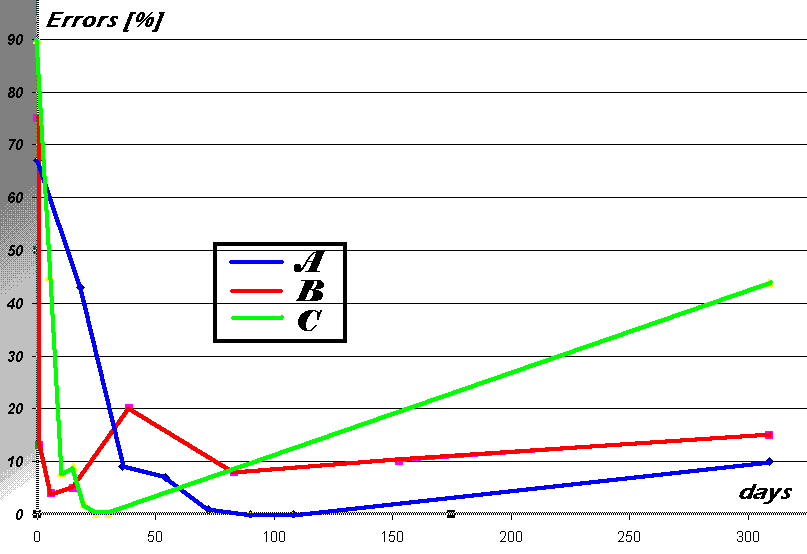
\includegraphics[width=0.8\textwidth]{images/three-group-repetition.png}
%   \caption{میانگین میزان خطای افراد در طول زمان در سه گروه آزمایشی}
%   \label{fig:three-group-repetition.png}
% \end{figure}


% وزنیاک انتظار داشت که روش B (فواصل افزایشی) بهترین نتیجه را بدهد. اما یافته‌ها متفاوت بود:
% \begin{itemize}
%     \item همان‌طور که در نمودار دیده می‌شود، گروه A در ابتدا خطای بیشتری داشت؛ یعنی تعداد زیادی از افعال فراموش می‌شد. اما در درازمدت میزان خطا کاهش پیدا کرد و پایدار ماند.
%     \item گروه C برعکس بود: بعد از ۳۰ روز و پایان شش مرور، تقریباً بدون خطا بود؛ اما با گذر زمان حافظه به سرعت افت کرد و خطاها به شدت افزایش یافتند.
% \end{itemize}

% نتیجه غافلگیرکننده بود: مرور ثابت هر ۱۸ روز (روش A) کارایی بهتری از مرور با بازه‌های افزایشی داشت. وزنیاک به این جمع‌بندی رسید که «هر فاصله‌ی افزایشی لزوماً مفید نیست» و باید الگویی بهینه برای زمان‌بندی تکرار پیدا کرد؛ الگویی که حتی از مرور منظم هم کارآمدتر باشد.

% برای مطالعهٔ بیشتر تحقیقات وزنیاک به فصل سوم
% مقالهٔ 
% \cite{ol}
% و یا
% \href{https://super-memory.com/english/ol/beginning.htm}{«شرح تحقیقاتی که منجر به روش \lr{SuperMemo} شد. تابع تقریبی بازه‌های بهینه»} 
%  مراجعه کنید.

برخلاف تصور اولیه که هر فاصله‌ی زمانی افزایشی برای مرور مناسب است، «وزنیاک» با طراحی آزمایشی نشان داد که نتایج ممکن است متفاوت باشد. او برای بررسی این موضوع، تعدادی فعل بی‌قاعده‌ی انگلیسی را به سه گروه تقسیم کرد و هر گروه را شش بار با فواصل زمانی متفاوت مرور کرد. برنامه‌ی زمانی این آزمایش در جدول~\ref{tbl:repetition_schedule} آمده است.


\begin{table}[h!]
    \centering
    \caption{برنامه زمانی مرور گروه‌های آزمایشی}
    \label{tbl:repetition_schedule}
    \begin{tabular}{|c|c|c|c|}
        \hline
        نوبت مرور & گروه A & گروه B & گروه C \\
        \hline
        ۱ & ۱۸ روز & ۱ روز & ۵ روز \\
        \hline
        ۲ & ۱۸ روز & ۵ روز & ۵ روز \\
        \hline
        ۳ & ۱۸ روز & ۹ روز & ۵ روز \\
        \hline
        ۴ & ۱۸ روز & ۲۴ روز & ۵ روز \\
        \hline
        ۵ & ۱۸ روز & ۴۴ روز & ۵ روز \\
        \hline
        ۶ & ۱۸ روز & ۷۰ روز & ۵ روز \\
        \hline
        مجموع & ۱۰۸ روز & ۱۵۳ روز & ۳۰ روز \\
        \hline
    \end{tabular}
\end{table}

قصد اصلی وزنیاک این بود که نشان دهد روش B (با فواصل افزایشی) بهترین نتیجه را به همراه دارد، اما نتایج که در شکل \ref{fig:three-group-repetition.png} مشاهده می‌کنید، متفاوت بود.

\begin{figure}[h!]
\centering
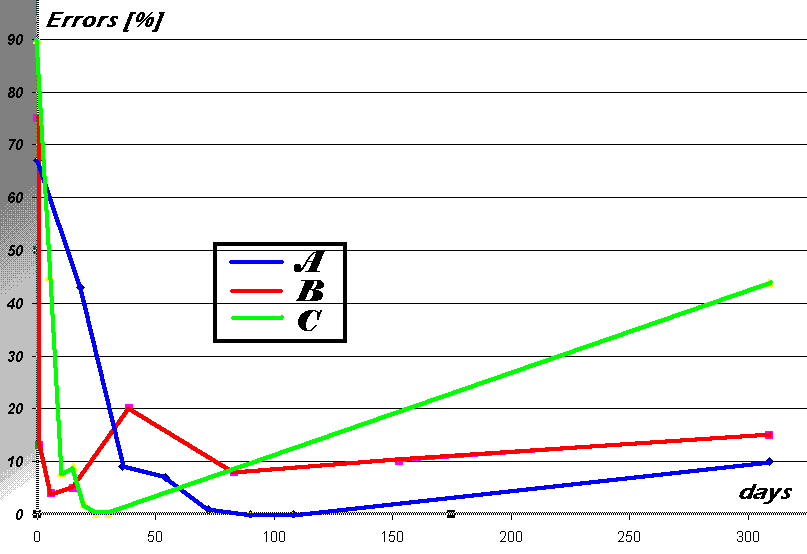
\includegraphics[width=0.8\textwidth]{images/three-group-repetition.png}
\caption{میانگین میزان خطای افراد در طول زمان در سه گروه آزمایشی}
\label{fig:three-group-repetition.png}
\end{figure}

همانطور که در نمودار دیده می‌شود، گروه A با وجود خطای بیشتر در ابتدا، در درازمدت عملکردی پایدارتر داشت، در حالی که گروه C پس از یک دوره کوتاه بدون خطا، به سرعت دچار فراموشی شد.
مهم تر از همه اینکه گروه A که با فواصل ثابت ۱۸ روز مرور می‌شد، در بلندمدت بهتر از گروه B با فواصل افزایشی عمل کرد.
این نتیجه غافلگیرکننده، وزنیاک را به این جمع‌بندی رساند که «هر فاصله‌ی افزایشی لزوماً مفید نیست» و یافتن الگویی بهینه برای زمان‌بندی تکرار،
که از فواصل زمان  ثابت‌هم کارآمدتر باشد، موضوع قابل توجهی است. 

برای مطالعهٔ بیشتر در مورد تحقیقات وزنیاک می‌توانید به فصل سوم مقالهٔ \cite{ol} و یا به لینک
\href{https://super-memory.com/english/ol/beginning.htm}{«شرح تحقیقاتی که منجر به روش \lr{SuperMemo} شد: تابع تقریبی بازه‌های بهینه»}
مراجعه کنید.

\chapter{الگوریتم لایتنر
\protect\footnote{\lr{Leitner}}
}

الگوریتم لایتنر، شناخته‌شده‌ترین الگوریتم در حوزه تکرار بافاصله است. این سیستم نوآورانه در دهه ۱۹۷۰ توسط \textbf{سباستین لایتنر}، روزنامه‌نگار و مروج علم آلمانی، توسعه یافت. او در کتاب تأثیرگذار خود با عنوان «این‌گونه باید آموخت»\footnote{\lr{So lernt man lernen}} که در سال ۱۹۷۲ منتشر شد، این روش را به مخاطبان گسترده‌تری معرفی کرد.
در ابتدا، این الگوریتم به صورت فیزیکی و با استفاده از \textbf{جعبه‌هایی با چند خانه} (معمولاً هفت خانه) پیاده‌سازی می‌شد. فلش‌کارت‌ها بر اساس میزان تسلط کاربر، بین این خانه‌ها جابجا می‌شدند. برای توضیحات بیشتر و یادگیری نحوه استفاده عملی از جعبه لایتنر به صورت فیزیکی، می‌توانید ویدیوی «\href{https://www.youtube.com/watch?v=JMoFwgdourI}{چطور از جعبه لایتنر استفاده کنیم؟}» را مشاهده کنید.
این الگوریتم با وجود سادگی، نتایج بسیار قابل قبولی ارائه می‌دهد و یک روش عالی برای آشنایی و یادگیری اصول تکرار بافاصله است.
به همین دلیل اول از همه به سراغ الگوریتم لایتنر می‌رویم.


\section{روش \lr{Leitner} چگونه کار می‌کند؟}

\begin{figure}[h!]
  \centering
  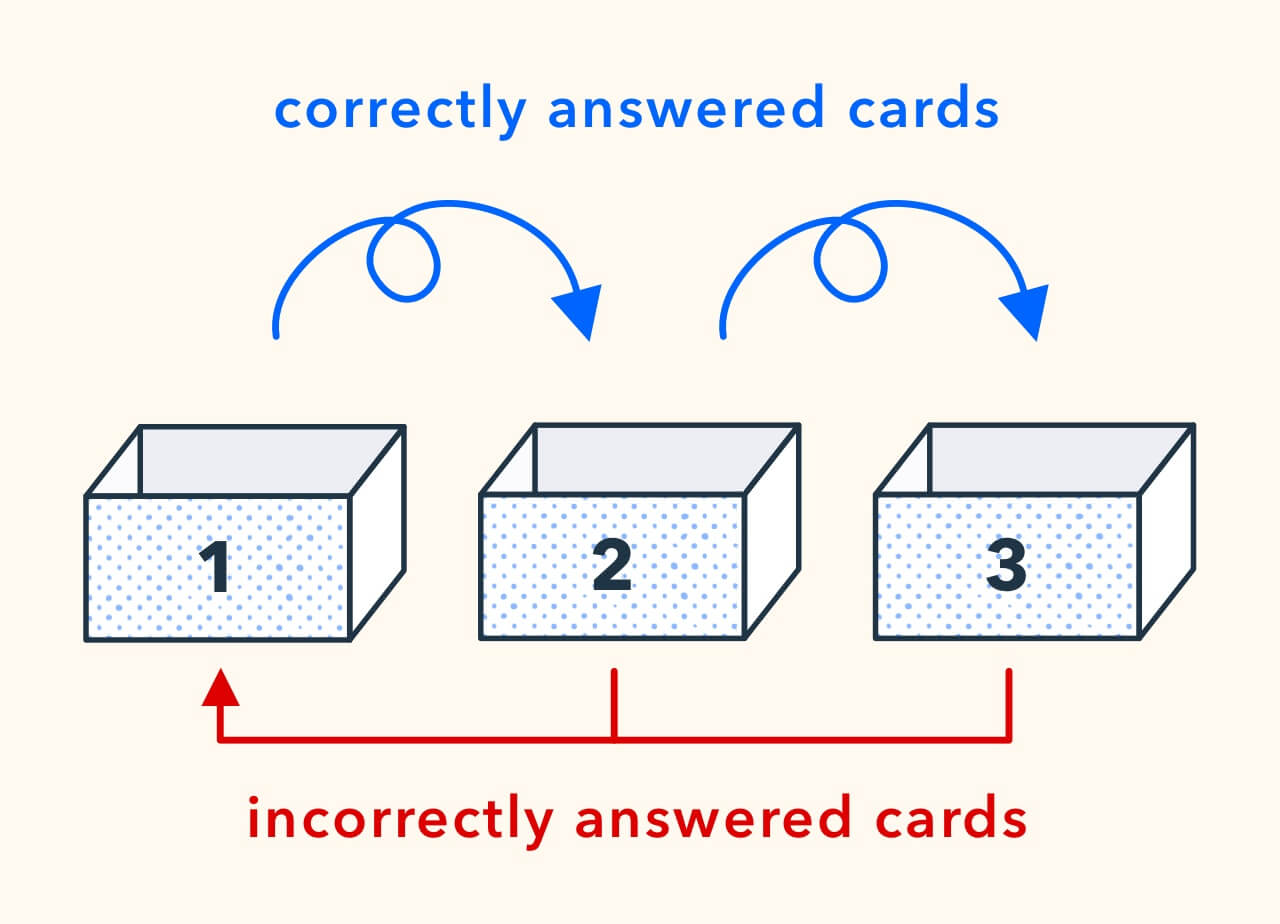
\includegraphics[width=0.8\textwidth]{images/leitner-overview.png}
  \caption{شمای کلی از روش لایتنر}
  \label{fig:leitner-overview}
\end{figure}

روش لایتنر بر اساس \textbf{تقسیم فلش‌کارت‌ها در خانه‌های مجزا} است. این خانه‌ها بر اساس میزان تسلط شما بر مطالب، دسته‌بندی می‌شوند. خانه‌های اولیه برای مرور بیشتر و خانه‌های پایانی برای مرور کمتر در نظر گرفته شده‌اند. اصول کلی این روش به صورت زیر است:


\begin{itemize}
    \item \textbf{حالت اولیه کارت‌ها:} همه فلش‌کارت‌ها در ابتدا در \textbf{خانه اول} قرار می‌گیرند.
    \item \textbf{جابه‌جایی کارت‌ها:} پس از هر بار مرور، اگر پاسختان صحیح باشد، کارت به خانه بعدی منتقل می‌شود. در غیر این صورت (پاسخ اشتباه)، کارت به \textbf{خانه اول} بازگردانده می‌شود تا بیشتر مرور شود.
    \item \textbf{فواصل زمانی مرور:} این روش نسخه‌های مختلفی دارد، اما رایج‌ترین آن‌ها \textbf{جعبه‌ای با هفت خانه} است. در این نسخه، مرور کارت‌ها در هر خانه به صورت تصاعدی افزایش می‌یابد؛ به عنوان مثال، خانه اول هر روز، خانه دوم هر دو روز، خانه سوم هر چهار روز و... مرور می‌شود.
\end{itemize}

به عنوان مثال فرض کنید فلش‌کارتی را از خانه سوم بیرون آورده‌اید که روی آن کلمه "\lr{garcon}" نوشته شده است، اما معنی آن را فراموش کرده‌اید. پس از مشاهده پاسخ (کلمه‌ای فرانسوی به معنی «پسر»)، کارت را به خانه اول برمی‌گردانید. \textbf{روز بعد}، چون خانه اول هر روز مرور می‌شود، دوباره "\lr{garcon}" را می‌بینید. اگر این بار پاسخ صحیح بدهید، کارت به خانه دوم منتقل می‌شود. اگر پاسخ اشتباه بدهید، در همان خانه اول باقی می‌ماند.

روند مرور ادامه پیدا می‌کند تا زمانی که کارت به خانه آخر برسد و شما به طور کامل بر آن مسلط شوید. وقتی کارت از خانه آخر خارج می‌شود، به این معنی است که آن مطلب به طور کامل یاد گرفته شده است و تا مدت زمان زیادی آن را فراموش نمی‌کنیم. بنابراین می‌توانیم آن کارت را از روند مطالعاتی خارج کنیم.

شبه کد پایتونی و ساده شده الگوریتم لایتنر را می‌توانید در قطعه کد زیر مشاهده کنید.

\begin{latin}
    
    \begin{lstlisting}[language=Python]
        DAY = 24 * 60 * 60    # seconds in a day (example)
        
        def get_cards_to_review(cards):
        """Return all cards that are due for review."""
        review_cards = []
        
        for card in cards:
        if card.review_date <= current_date:
        review_cards.append(card)
        
        return review_cards
        
        
        def mark_correct(card):
        """
        Update the card if the user answered correctly.
        - Increase the box number (spaced repetition level).
        - Schedule next review further in the future.
        """
        card.box_number += 1
        card.review_date = now() + (2 ** card.box_number) * DAY
        
        
        def mark_incorrect(card):
        """
        Update the card if the user answered incorrectly.
        - Reset box number.
        - Schedule review for tomorrow.
        """
        card.box_number = 0
        card.review_date = now() + 1 * DAY
    \end{lstlisting}
\end{latin}

\section{مزایای روش لایتنر}
روش لایتنر به طور خودکار و هوشمند نقاط ضعف شما را شناسایی و اولویت‌بندی می‌کند. کارت‌های دشوار در خانه‌های اولیه می‌مانند و بیشتر مرور می‌شوند، در حالی که مطالب آسان به خانه‌های آخر منتقل شده و کمتر تکرار می‌شوند. این سیستم با \textbf{منحنی فراموشی} تطابق بالایی دارد و سعی می‌کند که هر کارت قبل از فراموشی کامل، دوباره مرور شود و مدت زمان بیشتری در حافظه بماند.
در نتیجه، این روش به طور بهینه زمان مطالعه را مدیریت کرده و از مطالعه بیش از حد مطالبی که از قبل بر آن‌ها مسلط هستید، جلوگیری می‌کند.

\section{معایب روش لایتنر}
\begin{enumerate}
    \item \textbf{عدم توزیع هوشمندانه:} الگوریتم لایتنر، توزیع فلش‌کارت‌ها را بر اساس شروطی ساده انجام می‌دهد و همین موضوع می‌تواند منجر به نامنظم شدن حجم مطالعه در طول هفته شود. ممکن است در برخی روزها با حجم زیادی از کارت‌ها برای مرور مواجه شوید، در حالی که در روزهای دیگر، هیچ کارتی برای مطالعه نداشته باشید. برای مثال، اگر ۱۰ کارت جدید را در یک روز به سیستم اضافه کرده و به همه آن‌ها پاسخ درست دهید، این کارت‌ها به خانه دوم منتقل می‌شوند و دو روز بعد برای مرور مجدد ظاهر خواهند شد. در نتیجه، روز بعد هیچ کارتی برای مرور نخواهید داشت و این می‌تواند به برنامه‌ریزی شما لطمه بزند.
    \item \textbf{نادیده گرفتن سختی و آسانی پاسخ‌های درست:} این الگوریتم به میزان سختی یا آسانی یک پاسخ درست توجهی نمی‌کند. اگر مطلبی را به سختی به یاد آورید، آن را به خانه بعدی منتقل می‌کند؛ در حالی که اگر به مطلبی کاملاً مسلط باشید و به راحتی آن را به یاد آورید، باز هم همین کار را می‌کند. این عدم تفاوت‌گذاری باعث می‌شود که کارت‌های دشوار و آسان به یک شیوه مدیریت شوند و این می‌تواند کارایی سیستم را کاهش دهد و باعث شود بعضی کارت‌ها بیش‌از حد مرور شوند.
    \item \textbf{ضعف در تطبیق با وقفه‌های مطالعه:} روش لایتنر با وقفه‌های طولانی در مطالعه سازگاری خوبی ندارد. اگر برای مثال، یک کارت را در خانه اول قرار داده و پس از یک ماه به سراغ آن برگردید و جواب آن را بلد باشید، سیستم همچنان آن را به خانه دوم منتقل کرده و دو روز بعد به شما نشان می‌دهد. این در حالی است که وقتی بعد از یک ماه هنوز مطلب را به یاد دارید، نشان‌دهنده تسلط شما بر آن است و نیازی به مرور مجدد در فاصله زمانی کوتاه نیست. این نقص در بهینه‌سازی، زمان و انرژی شما را هدر می‌دهد.
\end{enumerate}

\chapter{الگوریتم \lr{SuperMemo}}

\textbf{سوپر ممو} 
یکی از پیشرفته‌ترین و پرکاربردترین الگوریتم‌های تکرار بافاصله است که توسط 
\textbf{پیوتر وُزنیـاک\footnote{Piotr Wozniak}}، پژوهشگر لهستانی، توسعه یافت. این الگوریتم به مرور زمان نسخه‌های مختلفی پیدا کرده (از \lr{SM-0} تا \lr{SM-18})
، اما نسخه‌ی معروف و پرکاربرد آن \textbf{\lr{SM-2}} است که هنوز هم اساس بسیاری از نرم‌افزارهای یادگیری 
مثل \lr{Anki}
\footnote{\lr{Anki} یک نرم افزار معروف برای مطالعه فلش‌کارت با استفاده از الگوریتم‌های با فاصله است.}
را تشکیل می‌دهد.همچنین یک نرم افزار به نام 
\lr{SuperMemo} وجود دارد که 
که توسط خود وُزنیـاک توسعه یافته است
و از نسخه‌های بالاتر این الگوریتم استفاده می‌کند.

\section{روش \lr{SuperMemo} چگونه کار می‌کند؟}
این روش پیچیدگی‌های بیشتری نسبت به روش لایتنر دارد و از چندین پارامتر برای تنظیم فواصل مرور استفاده می‌کند.
همچنین قواعد مرور نیز تفاوت‌هایی با روش لایتنر دارد.
\subsection{نحوه مرور و امتیازدهی به پاسخ‌ها}
هنگامی که یک فلش‌کارت را با روش \lr{SuperMemo} 
مرور می‌کنید، الگوریتم از شما می‌خواهد که عملکرد خود را بر اساس یک مقیاس درجه‌بندی 
(از ۰ تا ۵) 
ارزیابی کنید. وزنیاک این مقیاس را کیفیت پاسخ
\footnote{\lr{quality of response}}
 یا به اختصار
\lr{q}
 نامیده است.
 این امتیازدهی به الگوریتم کمک می‌کند تا بفهمد چقدر بر مطلب مسلط هستید و
سپس با استفاده از فرمول‌های پیچیده‌تر، 
فاصله زمانی بعدی را محاسبه می‌کند.
 در ادامه می‌توانید ببینید که هر کدام از این امتیازها به چه معنیست:

\begin{itemize}
    \item ۵ --~پاسخ کامل و بدون مشکل (\lr{perfect response})
    \item ۴ --~پاسخ صحیح با کمی تردید (\lr{correct response after a hesitation})
    \item ۳ --~پاسخ صحیح همراه با سختی زیاد (\lr{correct response recalled with serious difficulty})
    \item ۲ --~پاسخ اشتباه؛ اما یادآوری پاسخ صحیح آسان بود (\lr{incorrect response; where the correct one seemed easy to recall})
    \item ۱ --~پاسخ اشتباه؛ اما پاسخ صحیح به یاد آورده شد (\lr{incorrect response; the correct one remembered})
    \item ۰ --~فراموشی کامل (\lr{complete blackout})
\end{itemize}

\subsection{محاسبه فاصله زمانی مرور بعدی}
در روش 
\lr{SuperMemo}
فاصله زمانی با استفاده از فرمول بازگشتی زیر محاسبه می‌شود.
\begin{align}
I(0) &= 0 \\
I(1) &= 1\label{eq:interval1} \\
I(2) &= 6 \\
I(n) &= I(n-1) \times EF\label{eq:interval}
\end{align}

با توجه به فرمول محاسبه فاصله زمانی، می‌توانیم ببینیم که 
\textbf{فاصله زمانی برای مرور اول} برابر با ۱ روز و 
\textbf{برای مرور دوم} برابر با ۶ روز است. از اینجا به بعد، فاصله زمانی با توجه به 
\textbf{ضریب سهولت}
\footnote{\lr{Ease Factor}}
(\lr{EF})
کارت محاسبه می‌شود. به عنوان مثال، اگر ضریب سهولت یک کارت برابر با ۲ باشد، فاصله زمانی برای 
مرور سوم برابر با ۱۲ روز خواهد بود (۶ ضربدر ۲)
. اگر ضریب سهولت برابر با ۲٫۵ باشد، فاصله زمانی برای مرور سوم برابر با ۱۵ روز خواهد بود (۶ ضربدر ۲٫۵).
در نتیجه مرور اول و دوم برای همه کارت‌ها یکسان است، اما از مرور سوم به بعد، 
هر چه کارت آسان‌تر باشد، فاصله زمانی بیشتری برای مرور بعدی آن تعیین می‌شود.


همانطور که می‌بینیم
کیفیت پاسخ
(\lr{q})
تاثیر مستقیمی بر
بازه زمانی بعدی ندارد.
تاثیر این فاکتور از طریق
ضریب سهولت
به صورت غیرمستقیم اعمال می‌شود.
در قسمت
\ref{sec:sm-alg}
خواهیم دید که اگر \lr{q} کمتر از ۳ باشند،
\lr{r} به ۱ بازنشانی می‌شود،
 در نتیجه فاصله زمانی به ۱ روز کاهش می‌یابد.


\subsection{ضریب سهولت}
هر کارت یک ضریب مخصوص دارد که نشان‌دهنده‌ی میزان آسانی یا دشواری آن است.
 اگر کارتی برای شما دشوار باشد و اغلب نمره‌ی پایینی بدهید، 
 \lr{E-Factor} آن کاهش می‌یابد و مرورهای آینده نزدیک‌تر می‌شوند. اگر کارت آسان باشد، 
 \lr{E-Factor} آن بالا می‌رود و مرورها دورتر می‌شوند.

ضریب سهولت
در ابتدا برابر با ۲٫۵ تنظیم می‌شود و
 پس از هر بار مرور، این ضریب
 با استفاده از فرمول زیر محاسبه می‌شود:
\begin{align}
    EF' &= EF + (0.1 - (5-q) \times (0.08 + (5-q) \times 0.02))
\end{align}
که شکل کاهش یافتهٔ آن به صورت زیر است:
\begin{align}
    EF' &= EF - 0.8 + 0.28q - 0.02q^2\label{eq:ef-update}
\end{align}

توجه کنید که اگر کیفیت پاسخ برابر ۴ باشد، ضریب سهولت تغییری نمی‌کند.
همچنین طبق پژوهش‌های وزنیاک، ضریب سهولت نباید کمتر از ۱٫۳ باشد؛
زیرا در این صورت تعداد مرورها به شکل آزاردهنده‌ای افزایش پیدا می‌کند.
بنابراین اگر محاسبات منجر به ضریب سهولت کمتر از ۱٫۳ شود،
آن را برابر با ۱٫۳ در نظر می‌گیریم.

\subsection{الگوریتم \lr{SM-2}}\label{sec:sm-alg}
حال که با نحوهٔ محاسبه فاصله زمانی و ضریب سهولت آشنا شدیم،
می‌توانیم نسخهٔ کامل الگوریتم
\lr{SM-2}
که یکی از معروف‌ترین نسخه‌های \lr{SuperMemo} است را بررسی کنیم.

الگوریتم به این صورت عمل می‌کند:
\begin{enumerate}
    \item در ابتدا برای هر کارت ضریب سهولت را ۲٫۵، تعداد مرور
    (\lr{r}) را ۱ و آخرین بازه زمانی را برابر با ۰ قرار می‌دهیم.
    \item وقتی نوبت به مرور کارت رسید از کاربر می‌خواهیم که کیفیت پاسخ
    (\lr{q}) را از ۰ تا ۵ مشخص کند. سپس با توجه به مقدار \lr{q}، مراحل زیر را انجام می‌دهیم:
    \begin{enumerate}
        \item اگر کیفیت پاسخ
        (\lr{q}) کمتر از ۳ باشد:
        \begin{itemize}
            \item تعداد مرور
            (\lr{r}) را برابر به ۱ بازنشانی می‌کنیم.
            \item زمان مرور بعدی را
             با توجه به فرمول \ref{eq:interval1}
            یک روز بعد قرار می‌دهیم.
        \end{itemize}
        اگر کیفیت پاسخ
        (\lr{q}) برابر یا بیشتر از ۳ باشد:
        \begin{itemize}
            \item زمان مرور بعدی را با توجه به فرمول‌های
            \ref{eq:interval1} تا \ref{eq:interval}
            محاسبه می‌کنیم.
            \item تعداد مرور
            (\lr{r}) را یک واحد افزایش می‌دهیم.
        \end{itemize}
        \item ضریب سهولت را
        با توجه به فرمول \ref{eq:ef-update}
        به‌روزرسانی می‌کنیم و اگر کمتر از ۱٫۳ شد، آن را برابر با ۱٫۳ قرار می‌دهیم.
    \end{enumerate}
\end{enumerate}

شبه کد پایتونی و ساده شده الگوریتم \lr{SM-2} را می‌توانید در قطعه کد زیر مشاهده کنید.
\begin{latin}
    
    \begin{lstlisting}[language=Python]
        DAY = 24 * 60 * 60    # seconds in a day
        
        def get_cards_to_review(cards):
        """Return all cards that are due for review."""
        review_cards = []
        
        for card in cards:
        if card.review_date <= current_date:
        review_cards.append(card)
        
        return review_cards
        
        
        def mark_card(card, q):
        """
        Update the card based on the user's quality of response (q).
        q is an integer from 0 to 5.
        """
        if q < 3:
            # If the answer was incorrect or hard to recall
            card.repetition = 1
            card.review_date = now() + 1 * DAY
        else:
            # If the answer was correct
            if card.repetition == 1:
                interval = 1
            elif card.repetition == 2:
                interval = 6
            else:
                interval = card.interval * card.ease_factor
            
            card.repetition += 1
            card.review_date = now() + interval * DAY
            
        # Update ease factor
        card.ease_factor += (0.1 - (5 - q) * (0.08 + (5 - q) * 0.02))
        if card.ease_factor < 1.3:
            card.ease_factor = 1.3
    \end{lstlisting}
\end{latin}

پیاده‌سازی عملی و کامل این الگوریتم را می‌توانید در مخزن گیت‌هاب مربوط به این پروژه مشاهده کنید.

\section{مزایای روش \lr{SuperMemo}}
این الگوریتم نسخهٔ پیشرفته‌تری از روش لایتنر است و بیشتر مزایای روش لایتنر را دارد.
    علاوه بر این، با استفاده از امتیازدهی به پاسخ‌ها، می‌تواند فواصل زمانی را به صورت دقیق‌تری تنظیم کند و مشکل در نظر نگرفتن میزان سختی در پاسخ‌ها برطرف می‌شود.
این ویژگی باعث می‌شود که زمان مرور به نحو احسن مدیریت شود و مطالعه بیش از حد از مطالب آسان کاهش یابد.
همچنین تنوع در فواصل زمانی مرور باعث می‌شود که حجم مطالعه در طول هفته به شکل بهتری توزیع شود و از انباشتگی کارت‌ها در یک روز خاص جلوگیری شود.

\section{معایب روش \lr{SuperMemo}}
اگر چه این الگوریتم نسبت به روش لایتنر پیشرفته‌تر است، اما همچنان معایبی دارد که برطرف کردن آن‌ها نیازمند
الگوریتم‌های پیچیده‌تر است و همچنان محققان مشغول به پژوهش در این زمینه هستند.
از جمله معایب این روش می‌توان به موارد زیر اشاره کرد:

\begin{enumerate}
    \item \textbf{پیچیدگی امتیازدهی:} الگوریتم \lr{SuperMemo} نیازمند امتیازدهی دقیق از سوی کاربر است. این ممکن است برای برخی افراد دشوار باشد و باعث شود که امتیازها به صورت نادرست ثبت شوند.
    \item \textbf{عدم تطبیق با وقفه‌های مطالعه:} همانند روش لایتنر، این الگوریتم نیز با وقفه‌های طولانی در مطالعه سازگاری خوبی ندارد. اگر برای مثال، یک کارت را در فاصله زمانی کوتاه مرور کرده و سپس برای مدت طولانی به سراغ آن نروید، ممکن است الگوریتم نتواند به درستی تشخیص دهد که شما بر آن مطلب مسلط هستید یا خیر.
    \item \textbf{عدم شخصی سازی:} اگر چه این الگوریتم از امتیازدهی برای تنظیم فواصل زمانی استفاده می‌کند، اما همچنان از یک فرمول ثابت برای همه کاربران بهره می‌برد. این ممکن است باعث شود که الگوریتم نتواند به خوبی با سبک یادگیری و نیازهای خاص هر فرد سازگار شود.
    \item \textbf{عدم توجه به محتوی و نوع کارت:} این الگوریتم به محتوای کارت‌ها و نوع آن‌ها توجهی ندارد. برای مثال، یادگیری یک زبان جدید ممکن است نیازمند فواصل زمانی متفاوتی نسبت به یادگیری مفاهیم علمی باشد. این الگوریتم نمی‌تواند این تفاوت‌ها را در نظر بگیرد و ممکن است برای همه نوع مطالب به یک شکل عمل کند.
\end{enumerate}

% \chapter{عنوان فصل}

\chapter*{نتیجه‌گیری}

این پژوهش با هدف مقابله با چالش بنیادین فراموشی، به بررسی عمیق اصول و الگوریتم‌های \textbf{تکرار بافاصله} پرداخت. یافته‌ها به وضوح نشان می‌دهند که فلش‌کارت‌ها، بیش از یک ابزار ساده برای حفظ کردن هستند؛ آن‌ها ابزاری قدرتمند برای \textbf{یادگیری فعال} و بازیابی اطلاعات به شمار می‌روند. این روش، با استفاده از فواصل مرور هوشمندانه، به‌طور چشمگیری از اثرات \textbf{منحنی فراموشی} می‌کاهد و مطالب را از حافظه کوتاه‌مدت به حافظه بلندمدت منتقل می‌کند.

همان‌طور که مشاهده شد، الگوریتم‌های مختلفی برای پیاده‌سازی این سیستم‌ها وجود دارد؛ از روش ساده اما کارآمد \lr{Leitner} که اساس آن بر جابه‌جایی کارت‌ها در خانه‌های مجزا است، تا الگوریتم‌های پیشرفته‌تری چون \lr{SuperMemo} که با استفاده از داده‌های عملکردی کاربر، فواصل زمانی را به صورت پویا و کاملاً شخصی‌سازی شده تنظیم می‌کنند. در این میان، نتایج آزمایشات «وزنیاک» به ما آموخت که هر نوع تکرار بافاصله‌ای لزوماً کارآمد نیست و کلید موفقیت در یافتن الگوی بهینه و هوشمندانه برای زمان‌بندی مرور است.

در مجموع، این پژوهش تأکید می‌کند که بهینه‌سازی فرآیند یادگیری فراتر از مطالعه صرف است و در گرو انتخاب ابزارها و الگوریتم‌های مناسب قرار دارد. استفاده آگاهانه از فلش‌کارت‌ها و \textbf{الگوریتم‌های هوشمند} تکرار بافاصله، نه‌تنها زمان مطالعه را مدیریت می‌کند، بلکه به کاربر امکان می‌دهد تا بر نقاط ضعف خود تمرکز کرده و با کمترین تلاش، به بیشترین ماندگاری اطلاعات دست یابد. این رویکرد، در نهایت به تسلطی عمیق‌تر و پایدارتر بر دانش منجر خواهد شد.

% \chapter*{واژه‌نامه فارسی به انگلیسی}

% \chapter*{ واژه‌نامه انگلیسی به فارسی}

\begin{thebibliography}{MM}
    \begin{latin}
        \bibitem{ol}
            Woźniak, Piotr, and Edward Gorzelańczyk. "Optimization of repetition spacing in the practice of learning." Acta neurobiologiae experimentalis 54.1 (1994): 59-62.        
        \bibitem{20rules}
            P. Wozniak, ``Effective learning: Twenty rules of formulating knowledge'', 
            \url{https://super-memory.com/articles/20rules.htm}, 1999.
        \bibitem{ttk}
            Hunshamar, Asgeir. A Flashcard Based Web Application for Collective Learning and Peer Review Based Evaluation of Students. MS thesis. NTNU, 2021.
        \bibitem{how}
            Wissman, Kathryn T., Katherine A. Rawson, and Mary A. Pyc. "How and when do students use flashcards?." Memory 20.6 (2012): 568-579.
        \bibitem{fsrs}
            Ye, Junyao, Jingyong Su, and Yilong Cao. "A stochastic shortest path algorithm for optimizing spaced repetition scheduling." Proceedings of the 28th ACM SIGKDD conference on knowledge discovery and data mining. 2022.
        \bibitem{karl}
            Shu, Matthew, et al. "Karl: Knowledge-aware retrieval and representations aid retention and learning in students." arXiv preprint arXiv:2402.12291 (2024).
        \bibitem{trainable} 
            Settles, Burr, and Brendan Meeder. "A trainable spaced repetition model for language learning." Proceedings of the 54th annual meeting of the association for computational linguistics (volume 1: long papers). 2016.
        \bibitem{lstm}
            Pokrywka, Jakub, et al. "Modeling Spaced Repetition with LSTMs." CSEDU (2). 2023.

    \end{latin}
\end{thebibliography}

\begin{latin}
\begin{abstract}
This paper explores the mechanisms of memory enhancement through flashcards and the \textbf{spaced repetition} approach. First, the concept of the \textbf{forgetting curve} and its implications for learning are explained. Then, by introducing the characteristics of an effective flashcard, the cognitive principles behind this tool are examined. In the main section, the \textbf{key features of spaced repetition algorithms} (such as optimizing intervals and distributing review load) are discussed, and two important algorithms, \textbf{Leitner} and \textbf{SuperMemo}, are examined in detail. Finally, based on research findings and the experiments of \textbf{Wozniak}, this study emphasizes the importance of designing optimal algorithms for the effective management of the learning process.
\end{abstract}
\newpage
\thispagestyle{empty}
%Title page ---------------------------------------------
\begin{figure}
\centering

\includegraphics[height=2.5cm]{UT-Logo.pdf}
\end{figure}
\begin{center}

College of Science\\
School of Mathematics, Statistics, and Computer Science
\end{center}

\begin{center}
%%%%%%%%%%%%%
\end{center}

\begin{center}
\huge{An Introduction to Spaced Repetition Algorithms: How Flashcards Help Combat Forgetting?

}
\end{center}

\begin{center}
%%%
\end{center}

\begin{center}
\textbf{
Mohamamd Torabi
}
\end{center}

\begin{center}
Supervisor: Dr.\ Hedieh Sajedi
\end{center}

\vspace{3cm}
\begin{center}
A thesis submitted in partial fulfillment of the requirements for\\
the degree of B.Sc.\ in Computer Science
\end{center}

\begin{center}
2025
\end{center}

%\pagestyle{empty}
%\pagenumbering{}

\end{latin}

\end{document}
